\documentclass{beamer}
\mode<presentation>
\usepackage{amsmath}
\usepackage{amssymb}
\usepackage{bm}
%\usepackage{advdate}
\usepackage{adjustbox}
\usepackage{subcaption}
%\usepackage{enumitem}
\usepackage{enumerate}
\usepackage{multicol}
\usepackage{mathtools}
\usepackage{listings}
\usepackage{url}
\def\UrlBreaks{\do\/\do-}
\usetheme{Boadilla}
\usecolortheme{lily}
\setbeamertemplate{footline}
{
  \leavevmode%
  \hbox{%
  \begin{beamercolorbox}[wd=\paperwidth,ht=2.25ex,dp=1ex,right]{author in head/foot}%
    \insertframenumber{} / \inserttotalframenumber\hspace*{2ex} 
  \end{beamercolorbox}}%
  \vskip0pt%
}
\setbeamertemplate{navigation symbols}{}

\providecommand{\nCr}[2]{\,^{#1}C_{#2}} % nCr
\providecommand{\nPr}[2]{\,^{#1}P_{#2}} % nPr
\providecommand{\mbf}{\mathbf}
\providecommand{\pr}[1]{\ensuremath{\Pr\left(#1\right)}}
\providecommand{\qfunc}[1]{\ensuremath{Q\left(#1\right)}}
\providecommand{\sbrak}[1]{\ensuremath{{}\left[#1\right]}}
\providecommand{\lsbrak}[1]{\ensuremath{{}\left[#1\right.}}
\providecommand{\rsbrak}[1]{\ensuremath{{}\left.#1\right]}}
\providecommand{\brak}[1]{\ensuremath{\left(#1\right)}}
\providecommand{\lbrak}[1]{\ensuremath{\left(#1\right.}}
\providecommand{\rbrak}[1]{\ensuremath{\left.#1\right)}}
\providecommand{\cbrak}[1]{\ensuremath{\left\{#1\right\}}}
\providecommand{\lcbrak}[1]{\ensuremath{\left\{#1\right.}}
\providecommand{\rcbrak}[1]{\ensuremath{\left.#1\right\}}}
\providecommand{\rank}{\text{rank}}
\theoremstyle{remark}
\newtheorem{rem}{Remark}
\newcommand{\sgn}{\mathop{\mathrm{sgn}}}
\providecommand{\abs}[1]{\ensuremath{\left\vert #1 \right\vert}}
\providecommand{\res}[1]{\Res\displaylimits_{#1}} 
\providecommand{\norm}[1]{\lVert#1\rVert}
\providecommand{\mtx}[1]{\mathbf{#1}}
\providecommand{\mean}[1]{\overline{#1}}
\providecommand{\fourier}{\overset{\mathcal{F}}{ \rightleftharpoons}}
%\providecommand{\hilbert}{\overset{\mathcal{H}}{ \rightleftharpoons}}
\providecommand{\system}{\overset{\mathcal{H}}{ \longleftrightarrow}}
	%\newcommand{\solution}[2]{\vec{Solution:}{#1}}
%\newcommand{\solution}{\noindent \vec{Solution: }}
\providecommand{\dec}[2]{\ensuremath{\overset{#1}{\underset{#2}{\gtrless}}}}
\newcommand{\myvec}[1]{\ensuremath{\begin{pmatrix}#1\end{pmatrix}}}
\newenvironment{amatrix}[1]{%
  \left(\begin{array}{@{}*{#1}{c}|c@{}}
}{%
  \end{array}\right)
}
\let\vec\mathbf

\lstset{
%language=C,
frame=single, 
breaklines=true,
columns=fullflexible
}
\usepackage{listings}
\lstset{
  language=Python,
  basicstyle=\ttfamily\small,
  numbers=left,
  numberstyle=\tiny,
  breaklines=true,
  frame=single
}
%\numberwithin{equation}{section}

\title{Matgeo-1.7.5}
\author{AI25BTECH11019-Menavath Sai Sanjana}

\date{}

\begin{document}
\begin{frame}
\titlepage
\end{frame}

\begin{frame}
\frametitle{Question}
Find the value of p for which the points (-5,1),(1,p),(4,-2) are collinear
\end{frame}

\begin{frame}
\frametitle{Solution}

Let the points be

\begin{table}[h!]
\centering
\begin{tabular}{|c|c|}
\hline
\textbf{Point} & \textbf{Name} \\
\hline
$\myvec{-5 \\ 1}$ & $\vec{A}$ \\
\hline
$\myvec{1 \\ p}$ & $\vec{B}$ \\
\hline
$\myvec{4 \\ -2}$ & $\vec{C}$ \\
\hline
\end{tabular}
\caption{Variables Used}
\end{table}



The difference vectors are
\begin{align}
(\vec{B}-\vec{A}) &= \myvec{6 \\ p-1}, \\
(\vec{C}-\vec{A}) &= \myvec{9 \\ -3}.
\end{align}

\end{frame}
\begin{frame}
\frametitle{Solution(Continuation)}
Thus,
$
M^T = (\vec{B}-\vec{A} \;\; \vec{C}-\vec{A})^T
= \myvec{6 & p-1 \\ 9 & -3}.
$

Apply row operations to convert $M^T$ into upper triangular form.

\begin{align}
\myvec{6 & p-1 \\ 9 & -3} 
&\xrightarrow{R_2 \to R_2 - \tfrac{3}{2}R_1}
\myvec{6 & p-1 \\ 0 & -\tfrac{3}{2}(p+1)}.
\end{align}

For collinearity, $\operatorname{rank}(M^T)=1$.  
This happens when the second row is zero:
$
-\tfrac{3}{2}(p+1)=0.
$
\end{frame}

\begin{frame}
\frametitle{Conclusion}

$
p = -1
$

\bigskip

\textbf{Hence, the three points $A,B,C$ are collinear when $p=-1$.}
\end{frame}
\begin{frame}{Graphical Representation}

\begin{figure}[ht!]
    \centering
    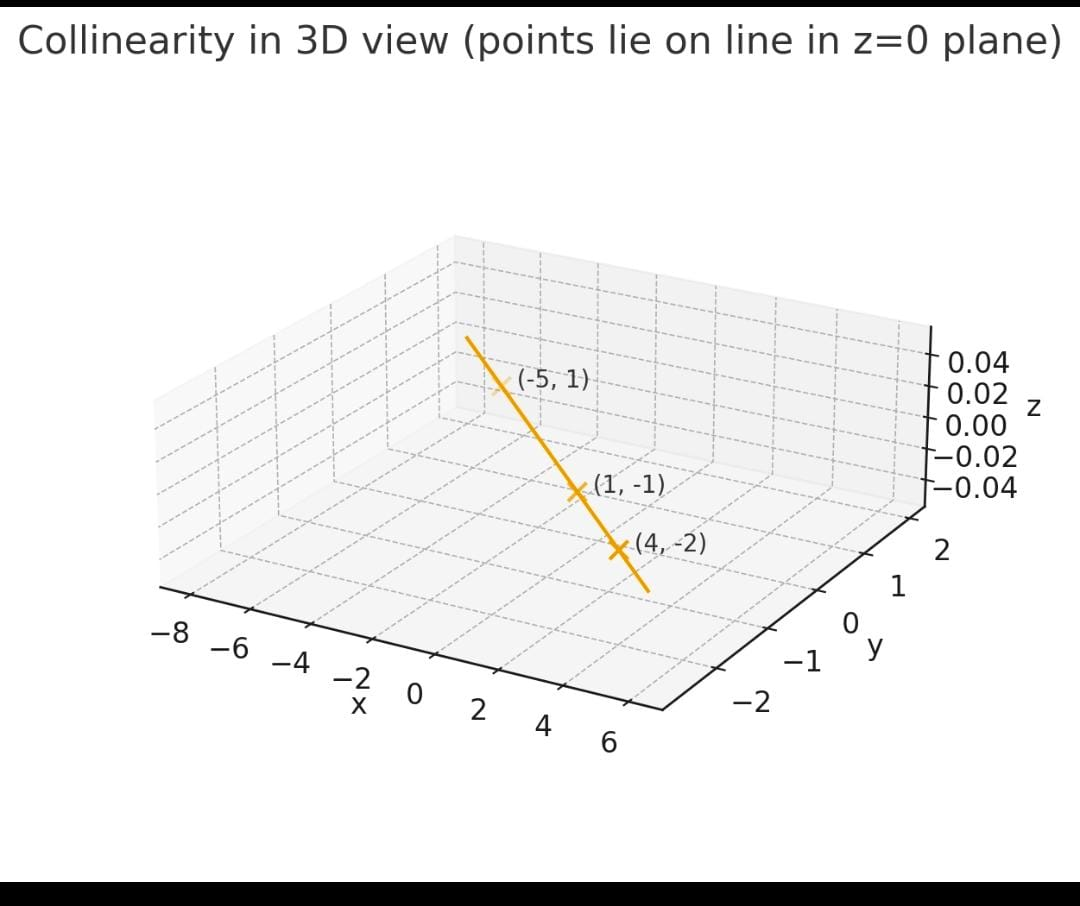
\includegraphics[width=0.7\textwidth]{matgeo-1.7.5.jpeg}
    \caption{}
    \label{fig:1.7.5.jpg}
\end{figure}

\end{frame}

\end{document}
